\section{Task Formulation and Methodology}
\label{sec:task-methodology}

\subsection{Prediction Task}

Our target is the DRAM-level Roofline Arithmetic Intensity (\rai) of a GPU kernel's \emph{first invocation}.
At prediction time, the LLM does not execute the program, collect profiler counters, or observe runtime traces.
Instead, it receives software artifacts and must infer the quantities from which \rai is derived.

We do not ask the model to emit \rai directly.
For each profiled sample, meaning one first-invocation kernel execution on one GPU, the model predicts seven values:
\begin{enumerate}[leftmargin=1.2em]
  \item grid size,
  \item block size,
  \item FP16 operation count,
  \item FP32 operation count,
  \item FP64 operation count,
  \item DRAM bytes read, and
  \item DRAM bytes written.
\end{enumerate}
We then derive \rai separately for each precision:
\[
\texttt{\rai}_{p}
=
\frac{\texttt{FLOP}_{p}}
     {\texttt{BytesRead} + \texttt{BytesWritten}},
\qquad
p \in \{\texttt{FP16}, \texttt{FP32}, \texttt{FP64}\}.
\]
This decomposition makes failures easier to interpret.
An incorrect launch configuration propagates into total work; an incorrect FLOP count indicates semantic or compiler-lowering errors; and an incorrect byte estimate indicates difficulty reasoning about DRAM-visible traffic.

We intentionally keep separate FP16/FP32/FP64 \rai values rather than collapsing mixed-precision kernels into a single scalar.
This matches the per-precision balance points used later for triage and makes compiler-injected FP16 work visible.
It also means that a kernel may have zero FP64 \rai but nonzero FP32 \rai, which we treat as a feature of the task rather than a modeling mistake.

\subsection{Input Evidence}

\begin{figure}[t]
  \centering
  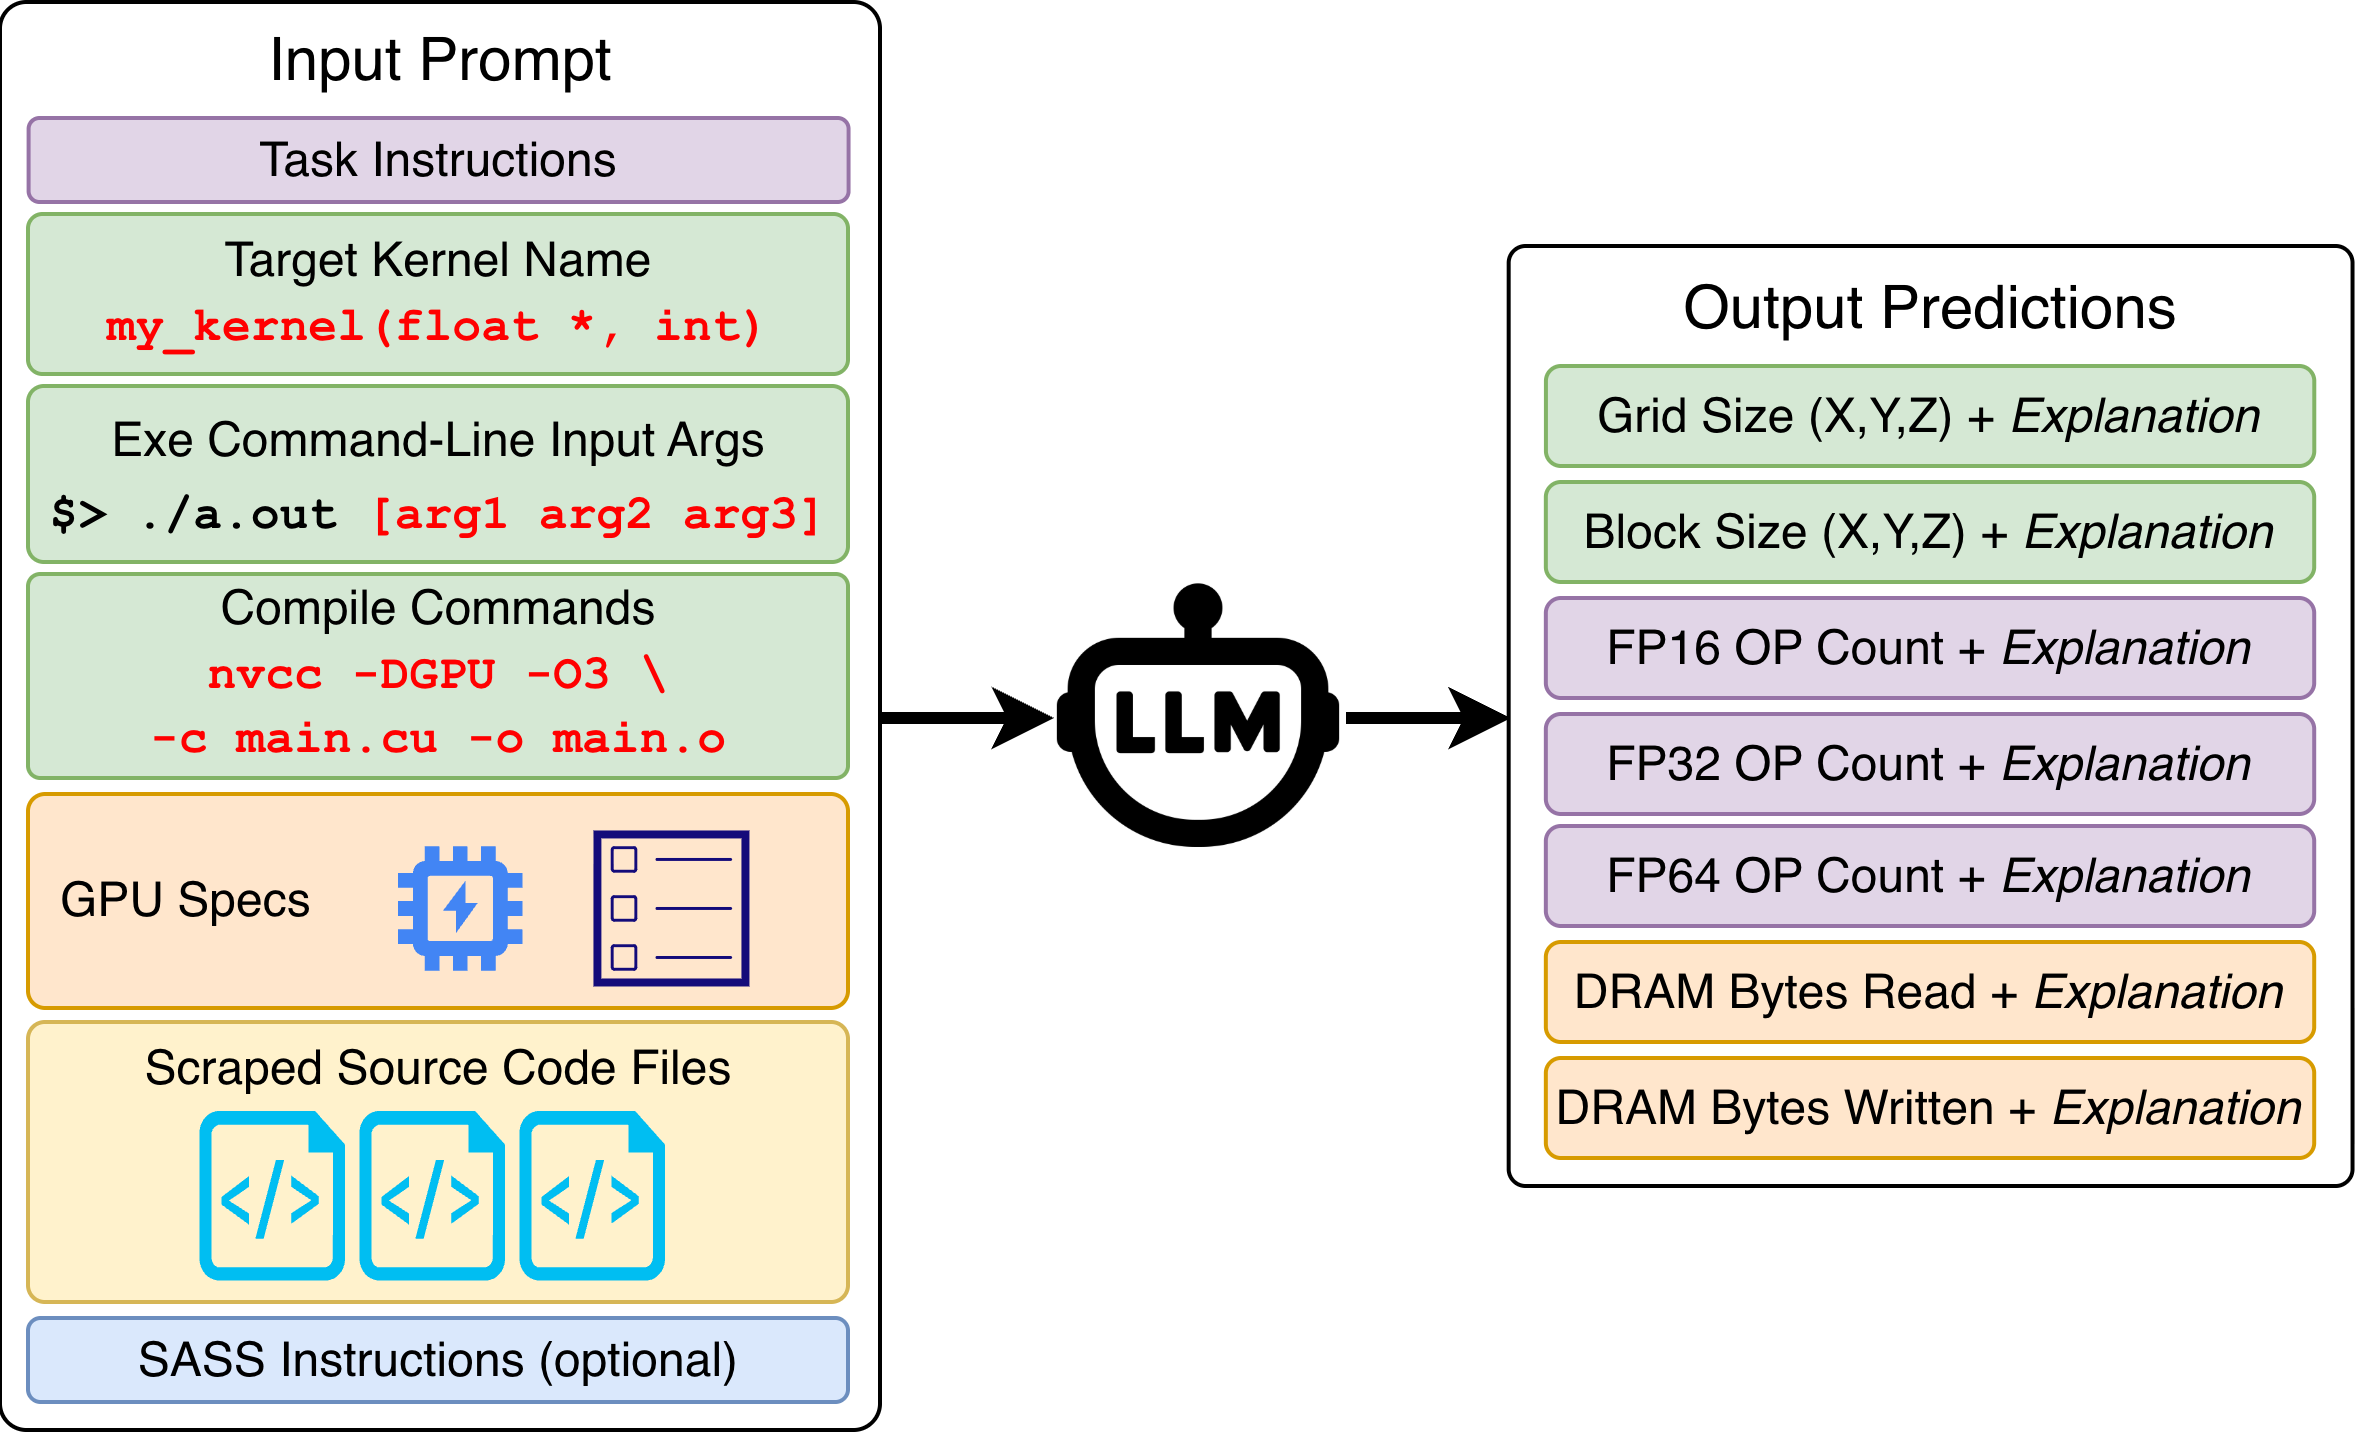
\includegraphics[width=\linewidth]{figures/prompting_pipeline.png}
  \caption{Per-kernel prompting workflow.
  Each query includes the target kernel name, source files, compile commands, runtime arguments, and GPU specifications.
  The \sourcesass setting adds target-kernel SASS sections and relevant helper routines so we can measure the value of post-compilation evidence.}
  \Description{A per-kernel prompt pipeline showing source files, build commands, runtime arguments, and GPU specifications as shared inputs, with SASS blocks added only in the source-plus-SASS setting before the model predicts launch sizes, FLOPs, and bytes.}
  \label{fig:prompting-pipeline}
\end{figure}

Figure~\ref{fig:prompting-pipeline} summarizes the evidence we provide to the model.
Every prompt contains the kernel identifier (mangled and demangled), relevant source files, compile commands, runtime arguments, and target-GPU specifications.
The \sourcesass configuration augments the same prompt with SASS sections for the target kernel and helper routines that may execute on its path.

The distinction between \sourceonly and \sourcesass is important.
\sourceonly corresponds to early development, code review, or agent planning when only pre-compilation artifacts are available.
\sourcesass still avoids target execution and profiling at prediction time, but it assumes target-specific compilation is possible, which is a materially different stage of the workflow.
We therefore treat \sourcesass as \emph{execution-free} rather than broadly ``hardware-free.'' 

The model returns a structured tool-call response containing the seven predicted quantities plus short explanations.
Those explanations are useful for sanity checking and for the later exploratory failure analysis, but they are not used to compute the reported metrics.

\subsection{Profiler-Derived Ground Truth}

Ground truth comes from an offline benchmark-building process, not from the prediction loop itself.
We profile each benchmark with NVIDIA Nsight Compute and retain the first invocation of the target kernel in each run.
We repeat the executable three times and average the retained first-invocation counters to reduce profiling noise.

The exact DRAM-traffic counters are \ctr{dram__bytes_read.sum} and \ctr{dram__bytes_write.sum}.
Floating-point counts are reconstructed from executed-operation counters:
\begin{itemize}[leftmargin=1.2em]
  \item FP32:
  \begin{quote}\raggedright\footnotesize
    \ctr{smsp__sass_thread_inst_executed_op_fadd_pred_on.sum.per_cycle_elapsed},
    \ctr{smsp__sass_thread_inst_executed_op_fmul_pred_on.sum.per_cycle_elapsed},
    \ctr{derived__smsp__sass_thread_inst_executed_op_ffma_pred_on_x2}.
  \end{quote}
  \item FP64:
  \begin{quote}\raggedright\footnotesize
    \ctr{smsp__sass_thread_inst_executed_op_dadd_pred_on.sum.per_cycle_elapsed},
    \ctr{smsp__sass_thread_inst_executed_op_dmul_pred_on.sum.per_cycle_elapsed},
    \ctr{derived__smsp__sass_thread_inst_executed_op_dfma_pred_on_x2}.
  \end{quote}
  \item FP16:
  \begin{quote}\raggedright\footnotesize
    \ctr{smsp__sass_thread_inst_executed_op_hadd_pred_on.sum.per_cycle_elapsed},
    \ctr{smsp__sass_thread_inst_executed_op_hmul_pred_on.sum.per_cycle_elapsed},
    \ctr{derived__smsp__sass_thread_inst_executed_op_hfma_pred_on_x4}.
  \end{quote}
\end{itemize}
We convert those per-cycle rates to total operation counts using
\ctr{smsp__cycles_elapsed.avg.per_second}
and
\ctr{gpu__time_duration.sum}.

These choices matter for scope.
Because bytes are counted at the DRAM interface, the task asks the model to predict \emph{DRAM-visible} traffic rather than raw source-level memory operations.
Writes that remain in the cache hierarchy until later are not immediately visible in the denominator.
Likewise, compiler-injected helper routines for division or transcendental functions contribute to the measured FLOP counts even when they are not obvious in source.
Those are precisely the cases where \sourcesass may add value.

\subsection{Why First Invocation and DRAM-Level \rai}

We make two deliberate simplifications.
First, we evaluate only the first invocation of each kernel, because repeated invocations introduce temporal cache reuse and cross-kernel interference that would substantially widen the reasoning space.
Second, we focus on DRAM-level \rai rather than a cache-aware Roofline.
This keeps the prediction target tied to one interpretable denominator while still exposing realistic sources of error such as L2 write-back behavior.

These simplifications narrow the claim.
The paper studies execution-free early triage for a first kernel invocation at the DRAM level; it does not claim to predict steady-state runtime behavior, cache-resident arithmetic intensity, or end-to-end application performance.
